\documentclass{report}

\usepackage[T1]{fontenc}
\usepackage[ngerman]{babel}
\usepackage[utf8]{inputenc}
\usepackage{lmodern}

\usepackage{amsmath}
\usepackage{amsthm}

\usepackage{graphicx}

% Randbreite reduzieren
\usepackage[paper=a4paper, left=25mm, right=25mm, top=25mm, bottom=25mm]{geometry}

% Entfernt das Einrücken von Absätzen 
\setlength{\parindent}{0pt}
\setlength{\parskip}{1em}

\title{Moderne Physik: Vorlesungsmitschrift}
\author{Daniel}
\date{\today}

\newcommand{\mdotvec}[1]{\dot{\vec{#1}}}
\newcommand{\mddotvec}[1]{\ddot{\vec{#1}}}
\newcommand{\msimplediff}[2]{\frac{\mathrm{d}#1}{\mathrm{d}#2}}
\newcommand{\mnorm}[1]{\left\lVert #1 \right\rVert}
\newcommand{\mabs}[1]{\left\lvert #1 \right\rvert}
\newcommand{\mvec}[1]{\begin{pmatrix} #1 \end{pmatrix}}
\newcommand{\md}{\mathrm{d}}
\newcommand{\mset}[1]{\left\{ #1 \right\}}

\DeclareMathOperator{\tr}{tr} % trace (Spur)

\begin{document}
	\maketitle
	\tableofcontents
	
	\chapter{Einleitung}

Verstehen im Gegensatz zur "`klassischen Physik"', entwickelt ab Anfang des 20. Jhd. Wichtigste Entwicklungen im 1. Viertel des Jhd.

Bis dahin (grob vereinfacht):
\begin{itemize}
	\item Newtonsche Mechanik
	\item Maxwells Elektrodynamik
\end{itemize}

\textbf{Paradigma}: alles im Prinzip berechenbar (Zeitentwicklung von System), solange die Anfangsbedingungen (alle $\vec{x}_i(t_0)$, $\dot{\vec{x}}_i(t_0)$, wobei $i =$ alle Punkte) bekannt sind.

\textbf{Aber}: Experimente zeigen immer mehr Widersprüche, zum Beispiel:
\begin{itemize}
	\item Michelson-Morley-Experiment: es gibt keinen "`Äther"', daraus hat sich die Spezielle Relativitätstheorie von Einstein (SRT) entwickelt
	\item Diskrete Energiespektren (Spektrallinien)
	\item Welleneigenschaft von Teilchen
	\item Teilcheneigenschaften von Lichtwellen
	\item Schwarzkörperstrahlung
	\item[$\Rightarrow$] das führte zur Quantenphysik 
\end{itemize}

Aufbau der Vorlesung:
\begin{enumerate}
	\item Klassische Mechanik
	\begin{itemize}
		\item Newtonsche Mechanik (sehr kurz)
		\begin{itemize}
			\item Entwicklung der formaleren analytischen Mechanik (Lagrange, Hamilton, Jacobi)
			\item erlaubt theoretische Diskussionen, z.B. Symmetrien und Erhaltungssätze; andere Konzepte, die in der Quantenmechanik (QM) eine Rolle spielen; "`Hamiltonoperator"'; kanonisch konjugierte Variable
		\end{itemize}
	\end{itemize}
	
	\item Relativität
	\begin{itemize}
		\item Symmetrie von Raum und Zeit
		\begin{itemize}
			\item daraus die Spezielle Relativität entwickeln (etwas losgelöst von klassischer Mechanik)
			\item formale Entwicklung, dann radikale Konsequenzen bestimmen
		\end{itemize}
	\end{itemize}
	
	\item Quantenmechanik
	\begin{itemize}
		\item wenig (?) Historie
		\item einfache eindimensionale Probleme 
		\begin{itemize}
			\item Schrödingergleichung
			\item Zusammenhang zur Wellenmechanik
		\end{itemize}
		\item Postulate der Quantenmechanik
		\item Symmetrien (?)
		\item Wasserstoffatom (System der Elemente)
		\item Identische Teilchen 
		\item Beispiele \dots
	\end{itemize}
\end{enumerate}
	\chapter{Klassische Mechanik}

\section{Abriss der Newtonschen Mechanik}

Problemstellung der klassischen Mechanik: Orte $\vec{r}_i$ und Geschwindigkeiten $\vec{v}_i$ zur Zeit $t$ gegeben für ein System von Massenpunkten mit $1 \le i \le N$ (also $N$ Massenpunkte).

Es wirken äußere Kräfte $\vec{F}$ und Kräfte zwischen den Teilchen $i$ und $j$ ($i \neq j$): $\vec{F}_{ij}$.

Wie lauten die \textbf{kinematischen Größen} $\vec{r}_i(t)$ und $\vec{v}_i(t) = \mdotvec{r}_i(t)$ (wobei $\mdotvec{r} = \msimplediff{\vec{r}}{t}$) für beliebige Zeiten $t$ danach?

Die kinematischen Größen $\vec{r}_i(t)$ (und $\mdotvec{r}_i(t)$) werden als Lösungen gewöhnlicher Differentialgleichungen gefunden; das sind die \textbf{Bewegungsgleichungen}.

Neben diesen kinematischen Größen gibt es die wichtigen Begriffe \textbf{Kraft}, \textbf{Masse}, \textbf{Impuls} und \textbf{Energie}.


\textbf{Kraft}: vektorielle Größe, meistens $\vec{F}$ (manchmal auch $\vec{K}$); ist immer die Ursache von Bewegung oder der Änderung von Bewegungszuständen, das heißt im Umkehrschluss: kräftefrei $\rightarrow$ Bewegung unverändert 
	
Das führt auf die \textbf{Newtonschen Gesetze}: 
\begin{description}
	\item[lex prima (Galileisches Trägheitsgesetz)] es gibt Initialsysteme, in denen ein kräftefreier Körper (= Massepunkt) ruht oder sich gradlinig gleichförmig bewegt
		
	\textbf{Definition}: Jeder Massepunkt setzt der Einwirkung von Kräften einen \textbf{Trägheitswiderstand} entgegen = Masse, oder besser: \textbf{träge Masse} (Formelzeichen: $m$)
		
	\textbf{Definition}: \textbf{Impuls} $\vec{p} = m \vec{v}$
		
	\item[lex secunda (Bewegungsgesetz)] $\mdotvec{p} = \vec{F}$; meistens ist $m$ unveränderlich, dann ist $\mdotvec{v} = \msimplediff{}{t} \vec{v} = \vec{a}$ und $\vec{F} = m \vec{a}$.
		
	\item[lex tertia (actio = reactio)] $\vec{F}_{ij} = - \vec{F}_{ji}$ 
	
	\begin{figure}
		\centering
		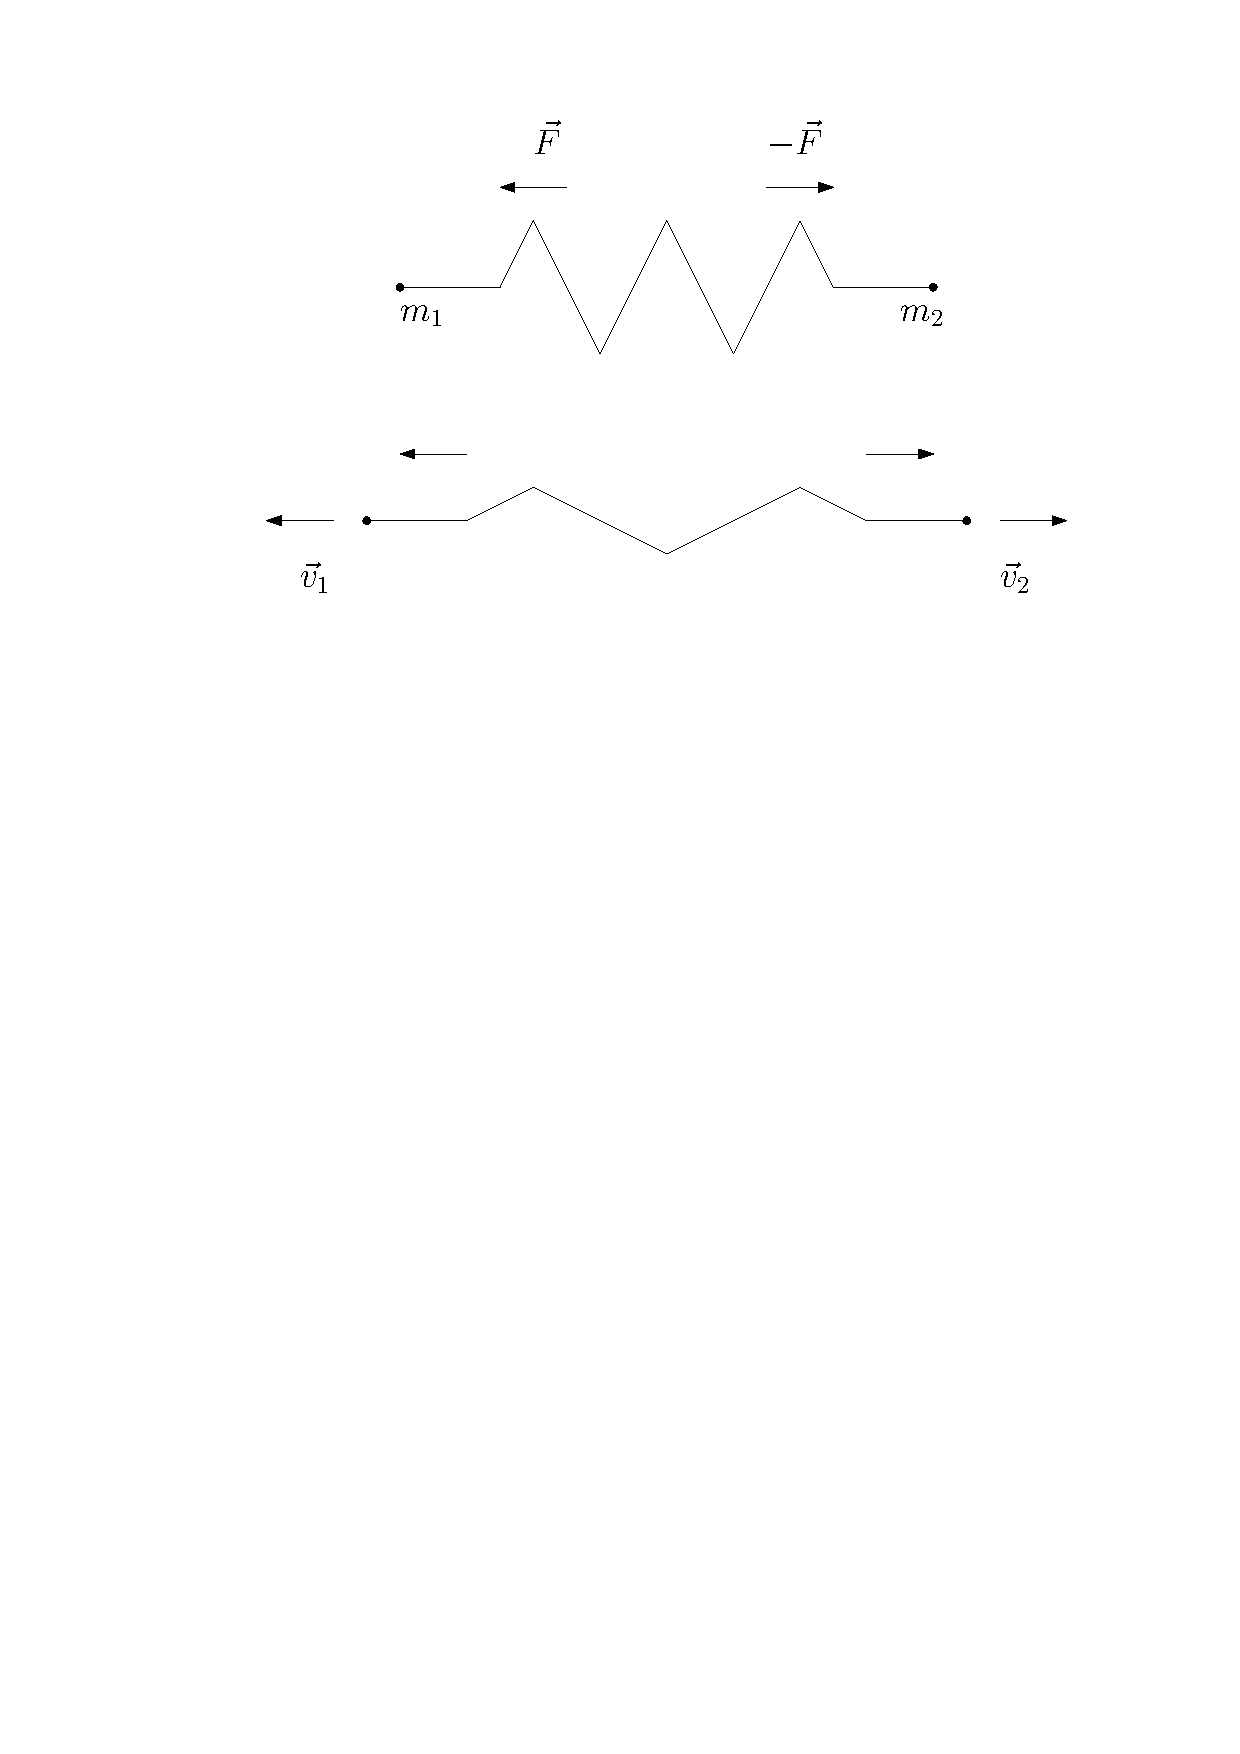
\includegraphics[scale=0.5]{figures/ch1/feder}
		\caption{actio = reactio bei einer Feder}
		\label{fig:ch1_feder}
	\end{figure}

	
	Beobachtung aus Abbildung \ref{fig:ch1_feder}: $\frac{v_1}{v_2} = \frac{m_2}{m_1}$, unabhängig von $\vec{F}$; das führt auf die Massendefinition
\end{description}

Wichtige Beispiele für Kräfte:

\begin{description}
	\item[Gravitationskraft (schwere Masse = träge Masse)] $\vec{F} = -\gamma \frac{M m}{r^2} \hat{r}$, wobei $\hat{r} = \frac{\vec{r}}{\mabs{\vec{r}}}$ und $\gamma$ die Gravitationskonstante ist
	
		Skizze
	
		Speziell auf der Erde: $r = r_e$, $M = M_e$, $\gamma$
		
		Damit $F = \underbrace{\gamma \frac{M_e}{r_e^2}}_{=: g} m = mg$ und $g \approx 9.81 m s^{-2}$; die Kraft zeigt nach unten, deswegen nur noch $F$ statt $\vec{F}$
	\item[Coloumbkraft] $\vec{F} = \frac{1}{4 \pi \epsilon_0} \frac{Q_1 Q_2}{r^2} \hat{r}$ zwischen elektrischen Ladungen $Q_1$ und $Q_2$; das sind zwei Zentralkräfte.
	\item[Lorentzkraft] $\vec{F} = e (\vec{E} + \vec{v} \times \vec{B})$: Ladung $e$, elektrisches Feld $\vec{E}$ und magnetisches Feld $\vec{B}$.
	\item[harmonischer Oszillator] lineare, stets negative (bezüglich der Bewegung) Kraft: $F = -\alpha \mabs{x}$
\end{description}

\textbf{Intertialsysteme / Nichtinertialsyseme}: In einem Inertialsystem: kräftefrei = gleichförmige Bewegung. 

Systeme $\Sigma$, $\Sigma'$ sind vollkommen gleichwertig, d.h. die physikalischen Gesetze sind forminvariant (kovariant) unter sogenannten Galilei-Transformationen. Das sind solche, die aus $\vec{r}' = \vec{r} + \vec{v}_0t$ machen, wenn sich $\Sigma$ und $\Sigma'$ mit $\vec{v}_0$ (=const) relativ zueinander bewegen. 

In \textbf{beschleunigten Systemen} gibt es sogenannte \textbf{Scheinkräfte};  zum Beispiel in rotierenden Systemen (Zentrifugalkraft, Corioliskraft).

Weitere Themen:
\begin{itemize}
	\item Schwingungsysteme (mit Dämpfung)
	\item Mehrere Massenpunkte (Eigenschwingungen)
	\item viel mehr Massenpunkte, "`starre Körper"'; Bewegung von Schwerpunkt + Rotation = "`Kreiselbewegung"'
\end{itemize}

\section{Lagrange-Mechanik}

Ausgangspunkt: Newton $m \mddotvec{r} = \vec{F}_i + \sum^N_{j \neq i} \vec{F}_{ij}$ für $i, j = 1, \dots, N$. $\vec{F}_i$ ist eine externe Kraft, $\vec{F}_{ij}$ sind Kräfte zwischen beteiligten Teilchen, paarweise. Damit: Problem vollständig formuliert, denn das sind $3N$ gewöhnliche Differentialgleichungen 2. Ordnung. Die sind im Prinzip lösbar mit den entsprechenden Anfangsbedingungen.

\textbf{Probleme}: 
\begin{itemize}
	\item Formulierung in Koordinaten $(x, y, z)_i$ ist meist zu kompliziert; damit wird die Lösung hoffnungslos.
	\item Meist Probleme mit eingeschränkter Geometrie. Zum Beispiel Perle auf kreisförmigem Draht (siehe Abbildung \ref{fig:ch1_perleaufdraht}). $(x, y, z)$ der Perle sinnvoll? $\phi$ viel geeigneter.
	\begin{figure}
		\centering
		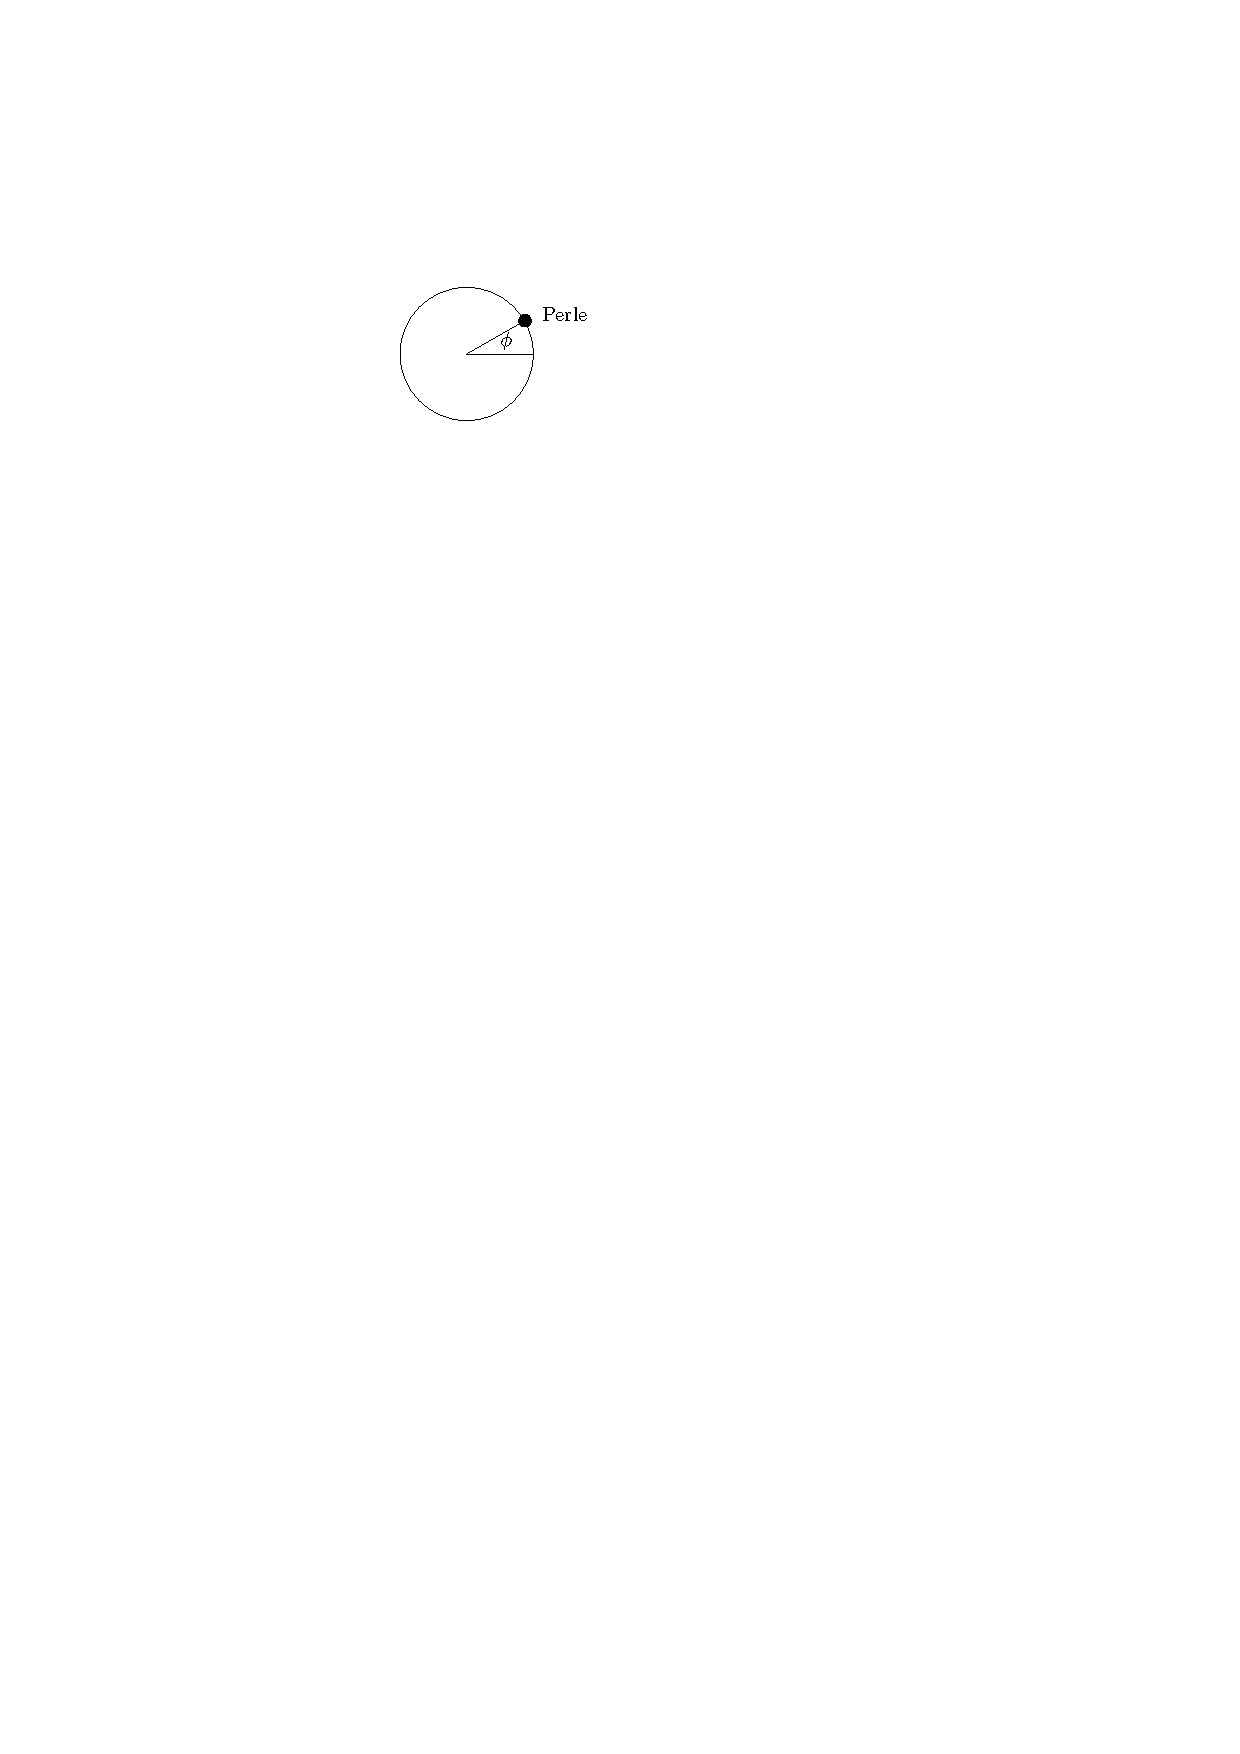
\includegraphics{figures/ch1/perleaufdraht}
		\caption{Die Position der Perle mit $\phi$ auszudrücken ist sinnvoller als mit $(x, y, z)$}
		\label{fig:ch1_perleaufdraht}
	\end{figure}
\end{itemize}

Die $\vec{F}_{ij}$ beschreiben geometrische Beziehungen auf komplizierte Weise $\rightarrow$ \textbf{Zwangskräfte} (im Beispiel die Kräfte, die die Perle auf dem Draht halten). Diese bewirken \textbf{Zwangsbedingungen}, die eigentlich direkt viel einfacher zu formulieren sind.

\textbf{Ziel der Lagrange-Mechanik}: Elimination der Zwangskräfte per verallgemeinerter Koordinaten (meist weniger als vorher)

Zwangsbedingungen sind:
\begin{itemize}
	\item A
	\begin{itemize}
		\item A1: holonom-shleronom(?): $\frac{\partial f_\nu}{\partial t} = 0$ mit $\nu = 1, \dots, p$ 
		\item A2: holonom-rheonom: $\frac{\partial f_\nu}{\partial t} \neq 0$ mit $\nu = 1, \dots, p$
	\end{itemize}
	\item B
	\begin{itemize}
		\item B1: als Ungleichungen $\rightarrow$ keine elimin... Bedingungen
		\item B2: differentielle Form: ???
	\end{itemize}
\end{itemize}


\textbf{Beispiele}:
\begin{itemize}
	\item Hantel (A1; siehe Abbildung \ref{fig:ch1_hantel}): $f(\vec{r}_i, \vec{r}_2) = 0$ und $(x_1 - x_2)^2 + (y_1 - y_2)^2 + (z_1 - z_2)^2 - l^2 = 0$.
	\begin{figure}
		\centering
		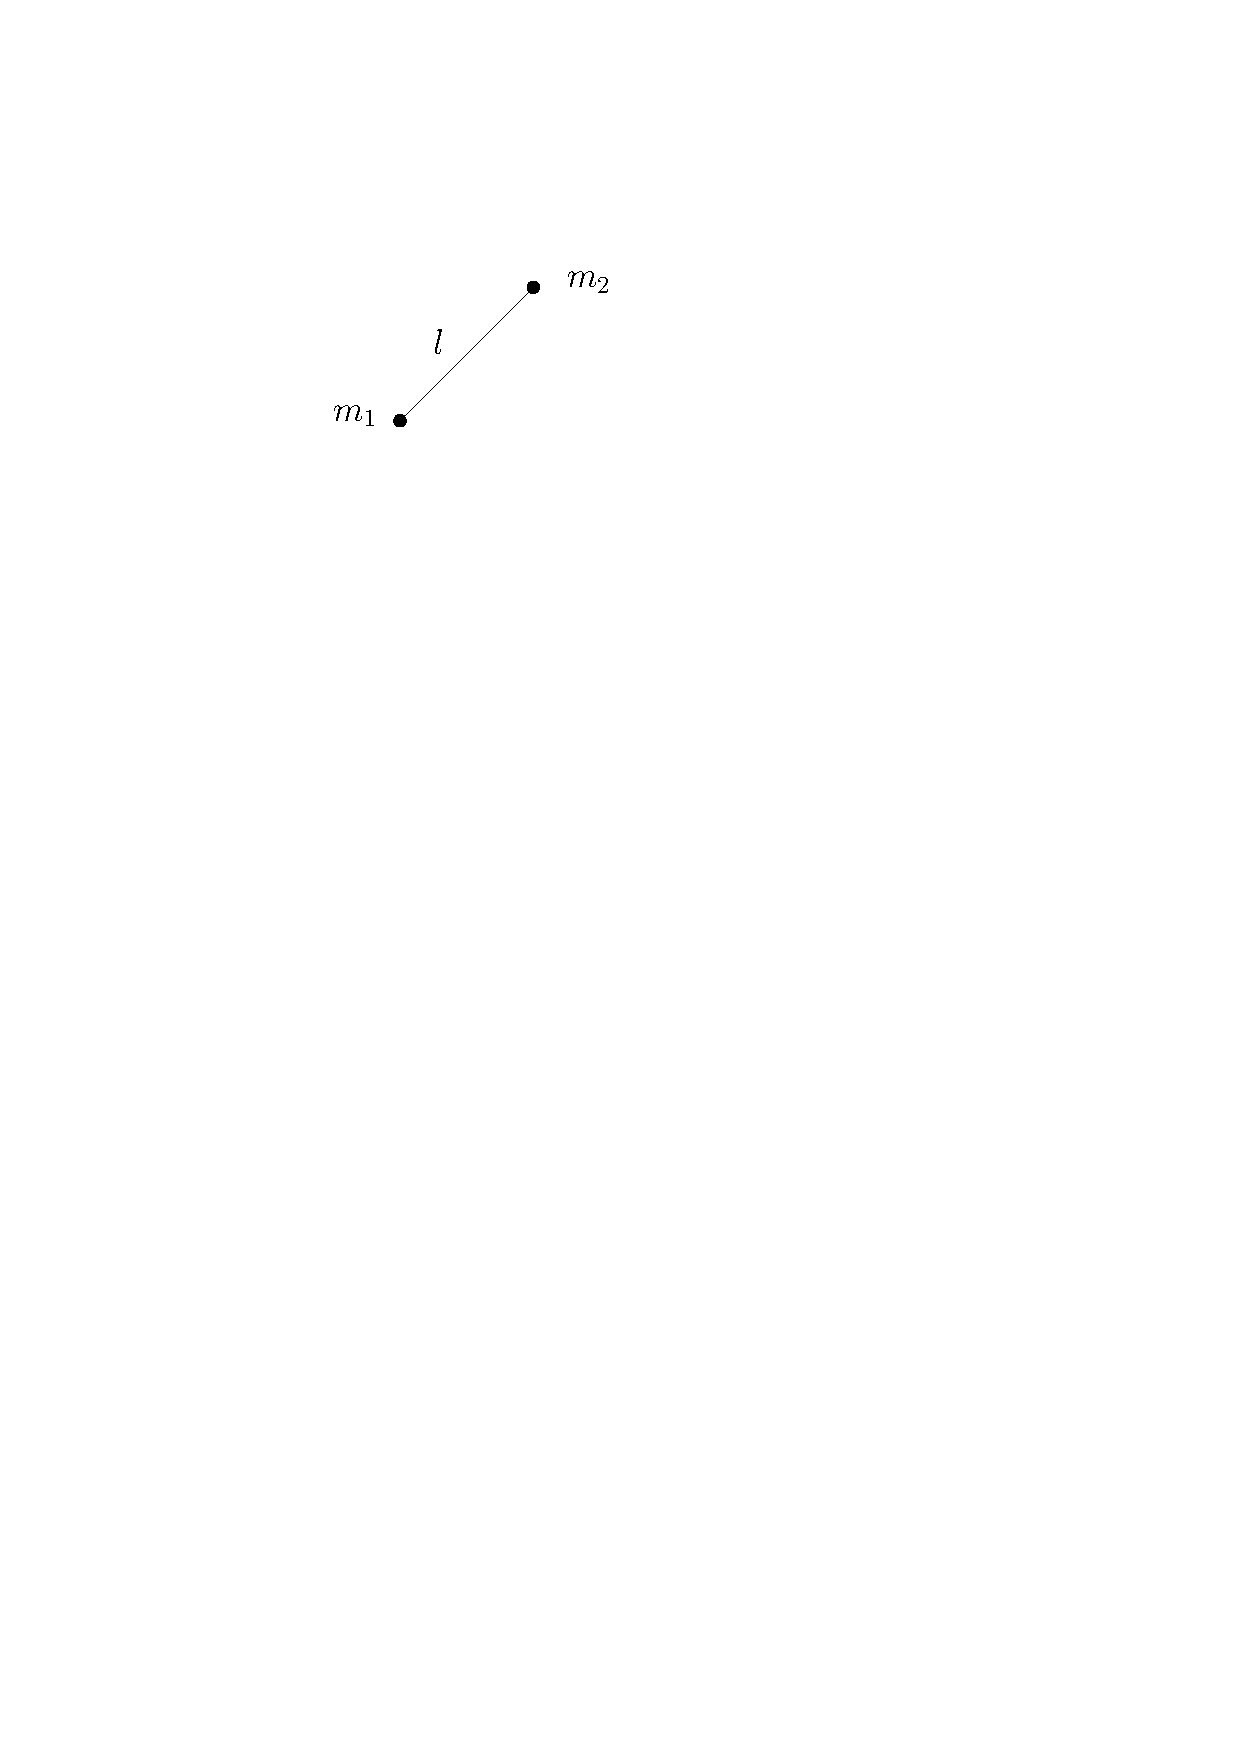
\includegraphics{figures/ch1/hantel}
		\caption{Eine Hantel der Länge $l$.}
		\label{fig:ch1_hantel}
	\end{figure}
	
	\item Ebene mit variablem Winkel (A2; siehe Abbildung \ref{fig:ch1_schiefeebene}): $\frac{z}{x} = \tan \phi(t)$
	\begin{figure}
		\centering
		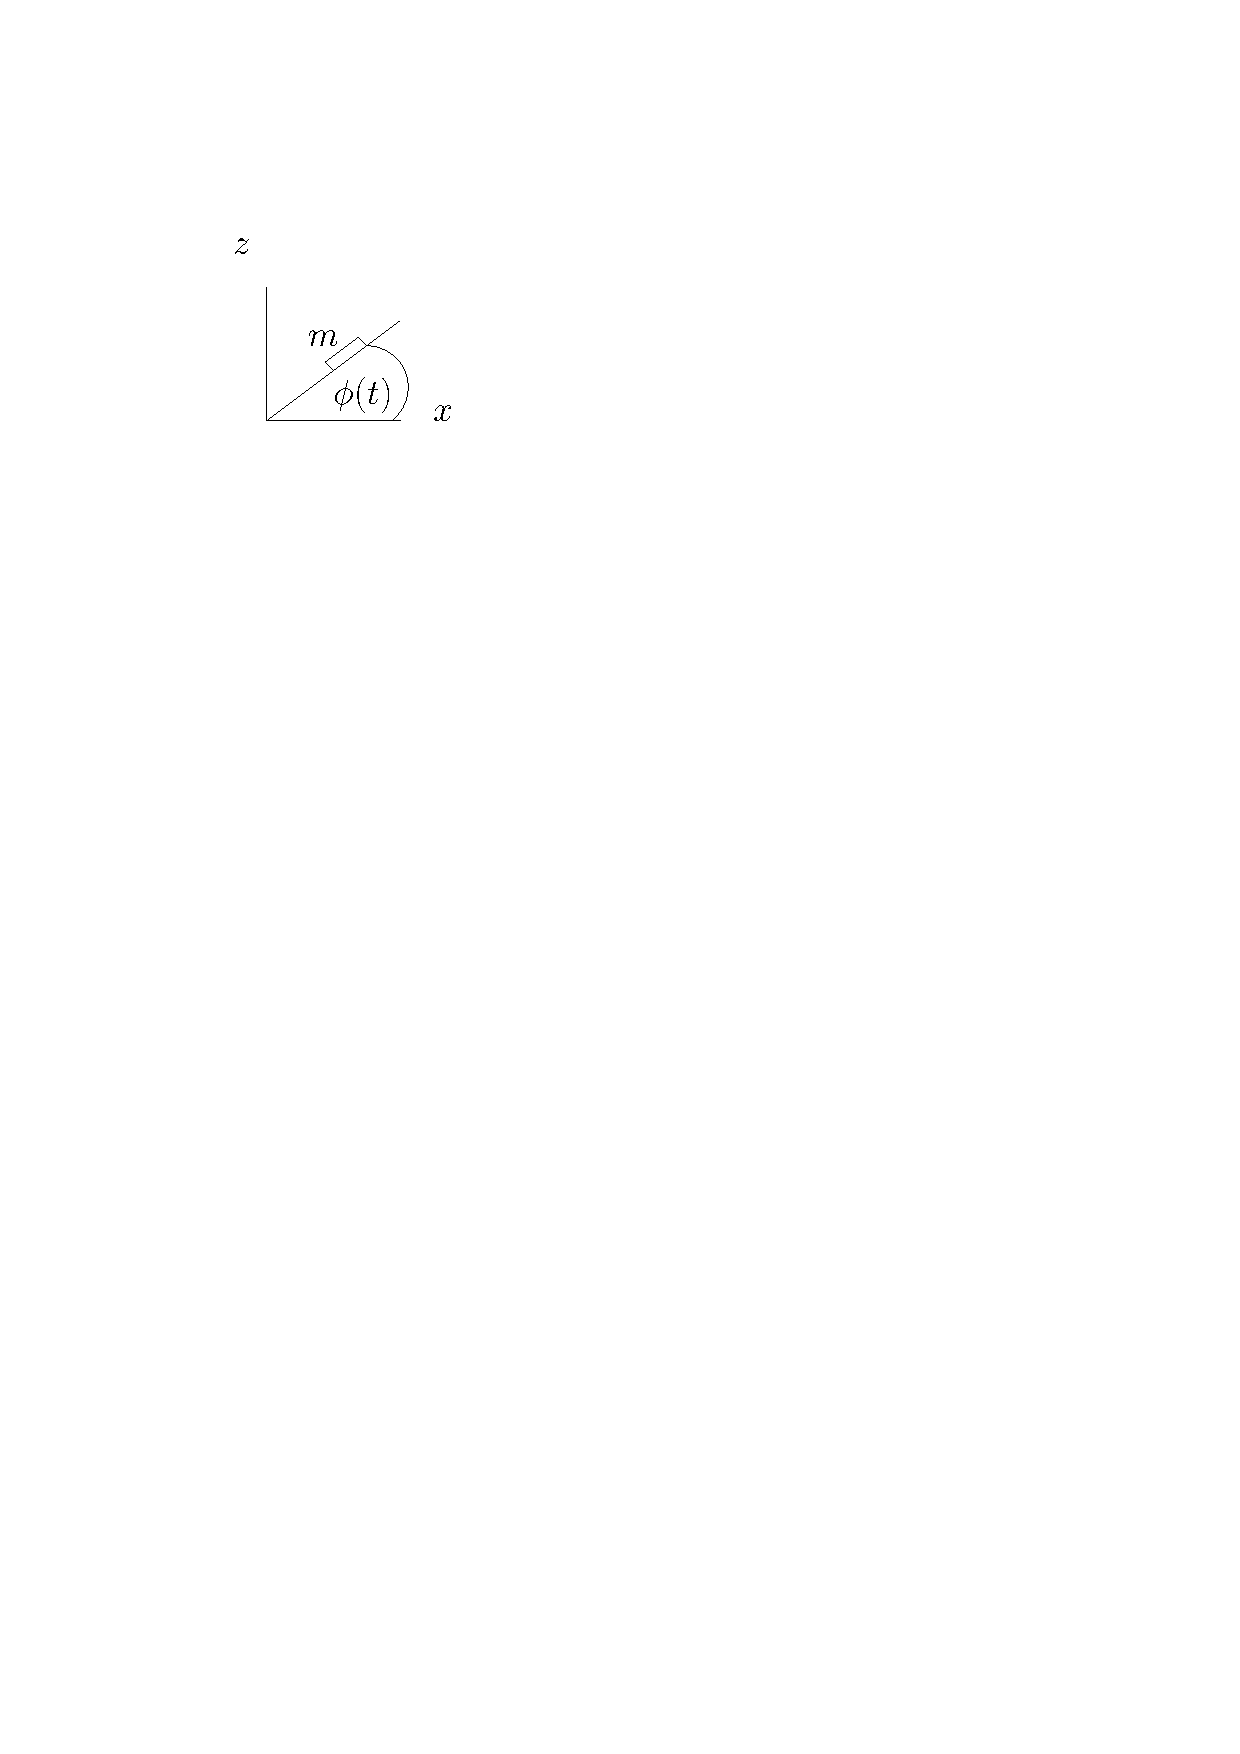
\includegraphics{figures/ch1/schiefeebene}
		\caption{Eine Hantel der Länge $l$.}
		\label{fig:ch1_schiefeebene}
	\end{figure}
\end{itemize}

Holonom: Reduktion der Freiheitsgrade $S = 3N - p$ bei $p$ holonomen Zwangsbedingungen $\rightarrow$ generalisierte Koordinaten, genannt $q_1, \dots, q_S$. Mit $\vec{r}_i = \vec{r}_i(q_1, \dots, q_S, t)$ sind Zwangsbedingungen implizit. Es gibt \textbf{keine} Beziehung $f(q_1, \dots, q_S, t) = 0$, d.h. es können keine Koordinaten eliminiert werden; $q_i$ unabhängig!

Schreibe $\vec{q} = (q_1, \dots, q_S)$ = Vektor aus dem $S$-dimensionalen Konfigurationsraum. Weiter sind $\dot{q}_1, \dots, \dot{q}_S$ die generalisierten Geschwindigkeiten.

\textbf{Bemerkung}: 
\begin{itemize}
	\item Mit $\vec{q}_0$, $\mdotvec{q}_0$ als Anfangsbedingungen sollte der Zustand zu jeder Zeit danach (oder davor) zu bestimmen sein.
	\item $\mset{q_S}$ ist nicht eindeutig, wohl aber die Anzahl $S$ (ergibt sich aus der physikalischen Problemstellung).
	\item Die $q_i$ haben eine nicht vorgegebene Dimension (müssen keine Längen sein, können z.B. auch Winkel sein). Eventuell ist die physikalische Bedeutung der $q_i$ nicht offensichtlich. Meistens sind es aber geometrische Größe.
\end{itemize}

\textbf{Beispiele}:
\begin{enumerate}
	\item Teilchen auf einer Kugeloberfläche (siehe Abbildung \ref{fig:ch1_kugel}) $\vec{r} = (x, y, z)$; $p = 1$ 
	
	\textbf{Zwangsbedingung}: $x^2 + y^2 + z^2 - R^2 = 0$, also $S = 3 - 1 = 2$. 
	
	$2$ quadratische Koordinaten, z.b. Winkel $q_1 = \nu$, $q_2 = \phi$
	\begin{figure}
		\centering
		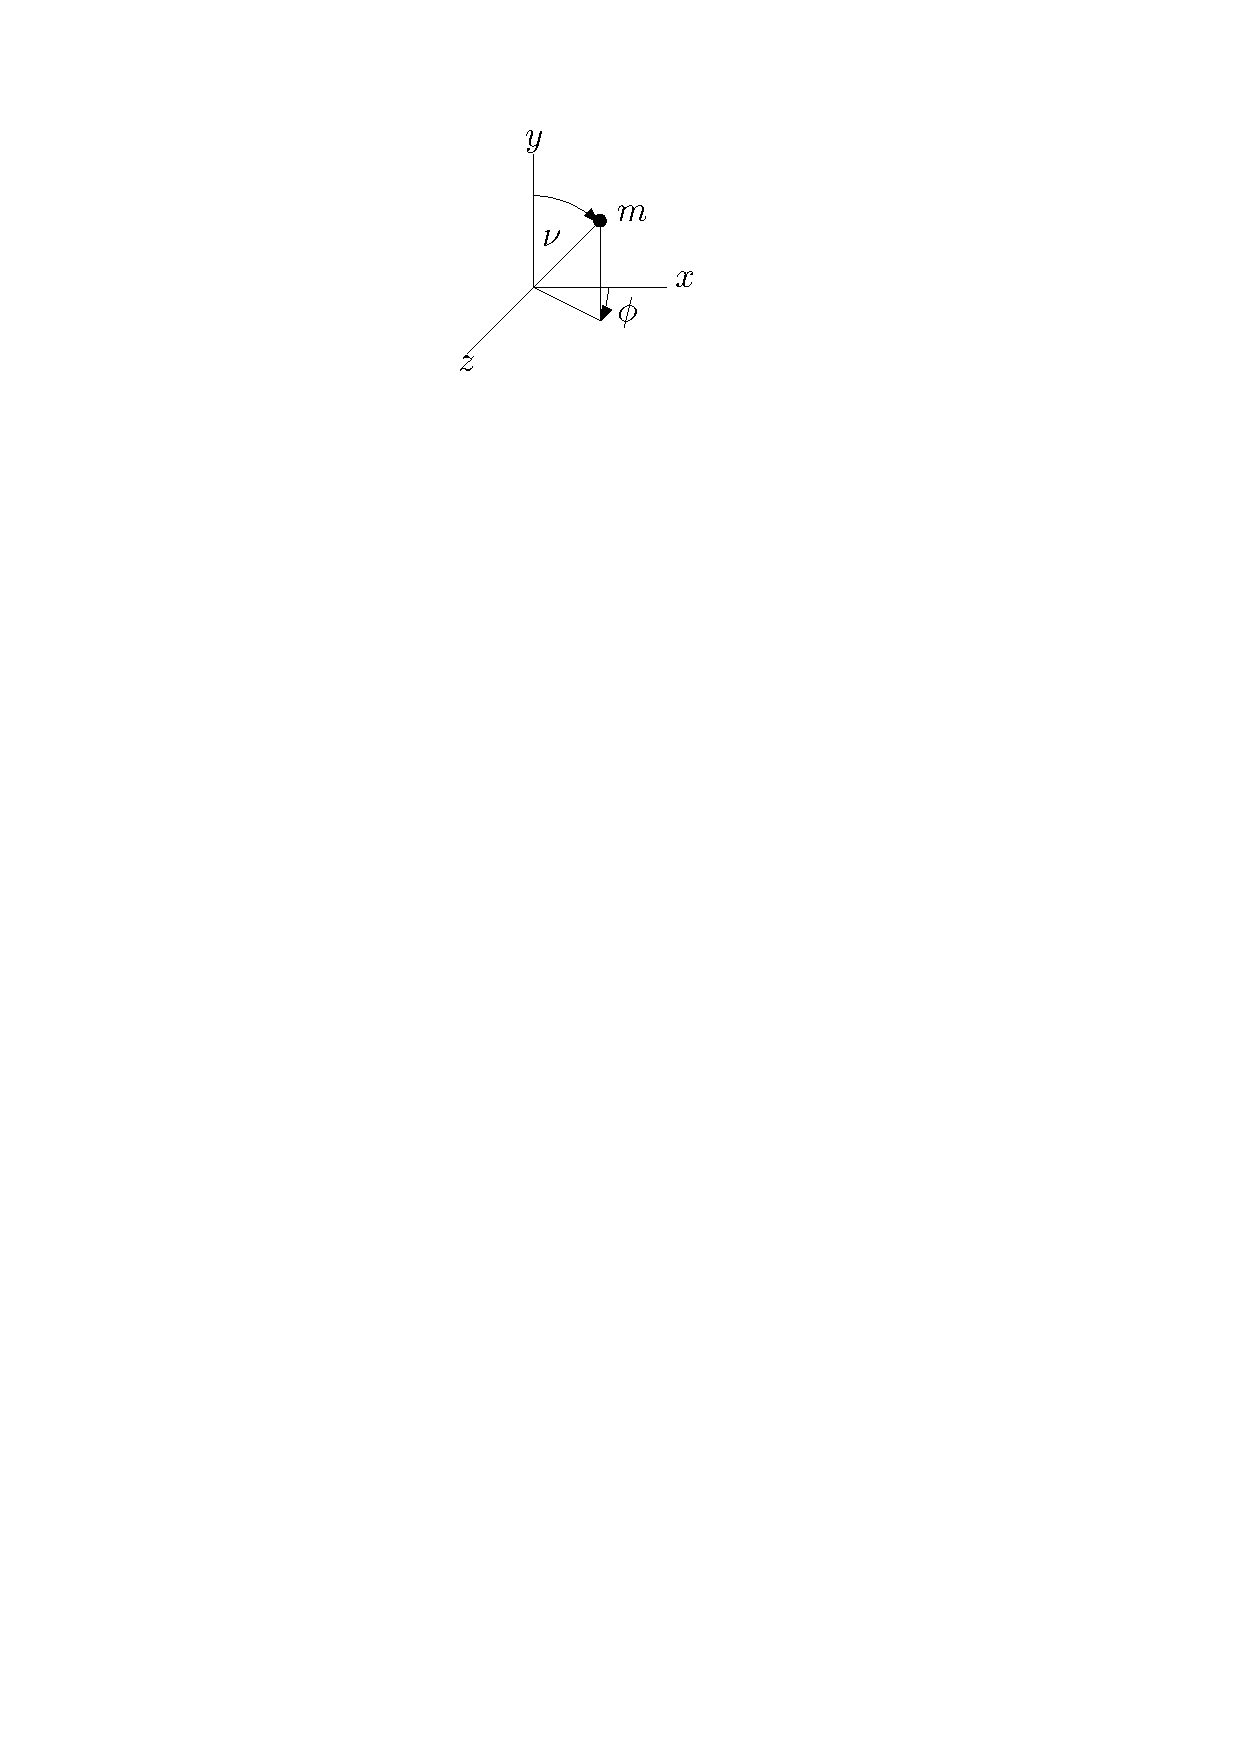
\includegraphics{figures/ch1/kugel}
		\caption{Kugel}
		\label{fig:ch1_kugel}
	\end{figure}
	
	$x = R \sin q_1 \cos q_2$, $y = R \sin q_1 \sin q_2$, $z = R \cos q_1$ $\rightarrow$ Zwangsbedingungen sind implizit, denn bei dieser Beschreibung immer erfüllt
	
	\item Doppelpendel (siehe Abbildung \ref{fig:ch1_doppelpendel}): zwei Massen $m_1$, $m_2$ = $6$ Freiheitsgrade
	
	vier davon sind holonom-shleronom: $z_1 = z_2 = ?$, $x_1^2 + y_1^2 - l_1^2 = 0$, $(x_2 - x_1)^2 + (y_2 - y_1)^2 - l_2^2 = 0$
	
	Wie viel generalisierte Koordinaten? $S = 6 - 4 = 2$ $\rightarrow$ zum Beispiel $q_1 = \nu_1$, $q_2 = \nu_2$
	
	$x_1 = l_1 \cos q_1$, $y_1 = l_1 \sin q_1$, $z_1 = 0$
	
	$x_2 = l_1 \cos q_1 + l_2 \cos q_2$, $y_2 = l_1 \sin q_1 + l_2 \sin q_2$, $z_2 = 0$
	\begin{figure}
		\centering
		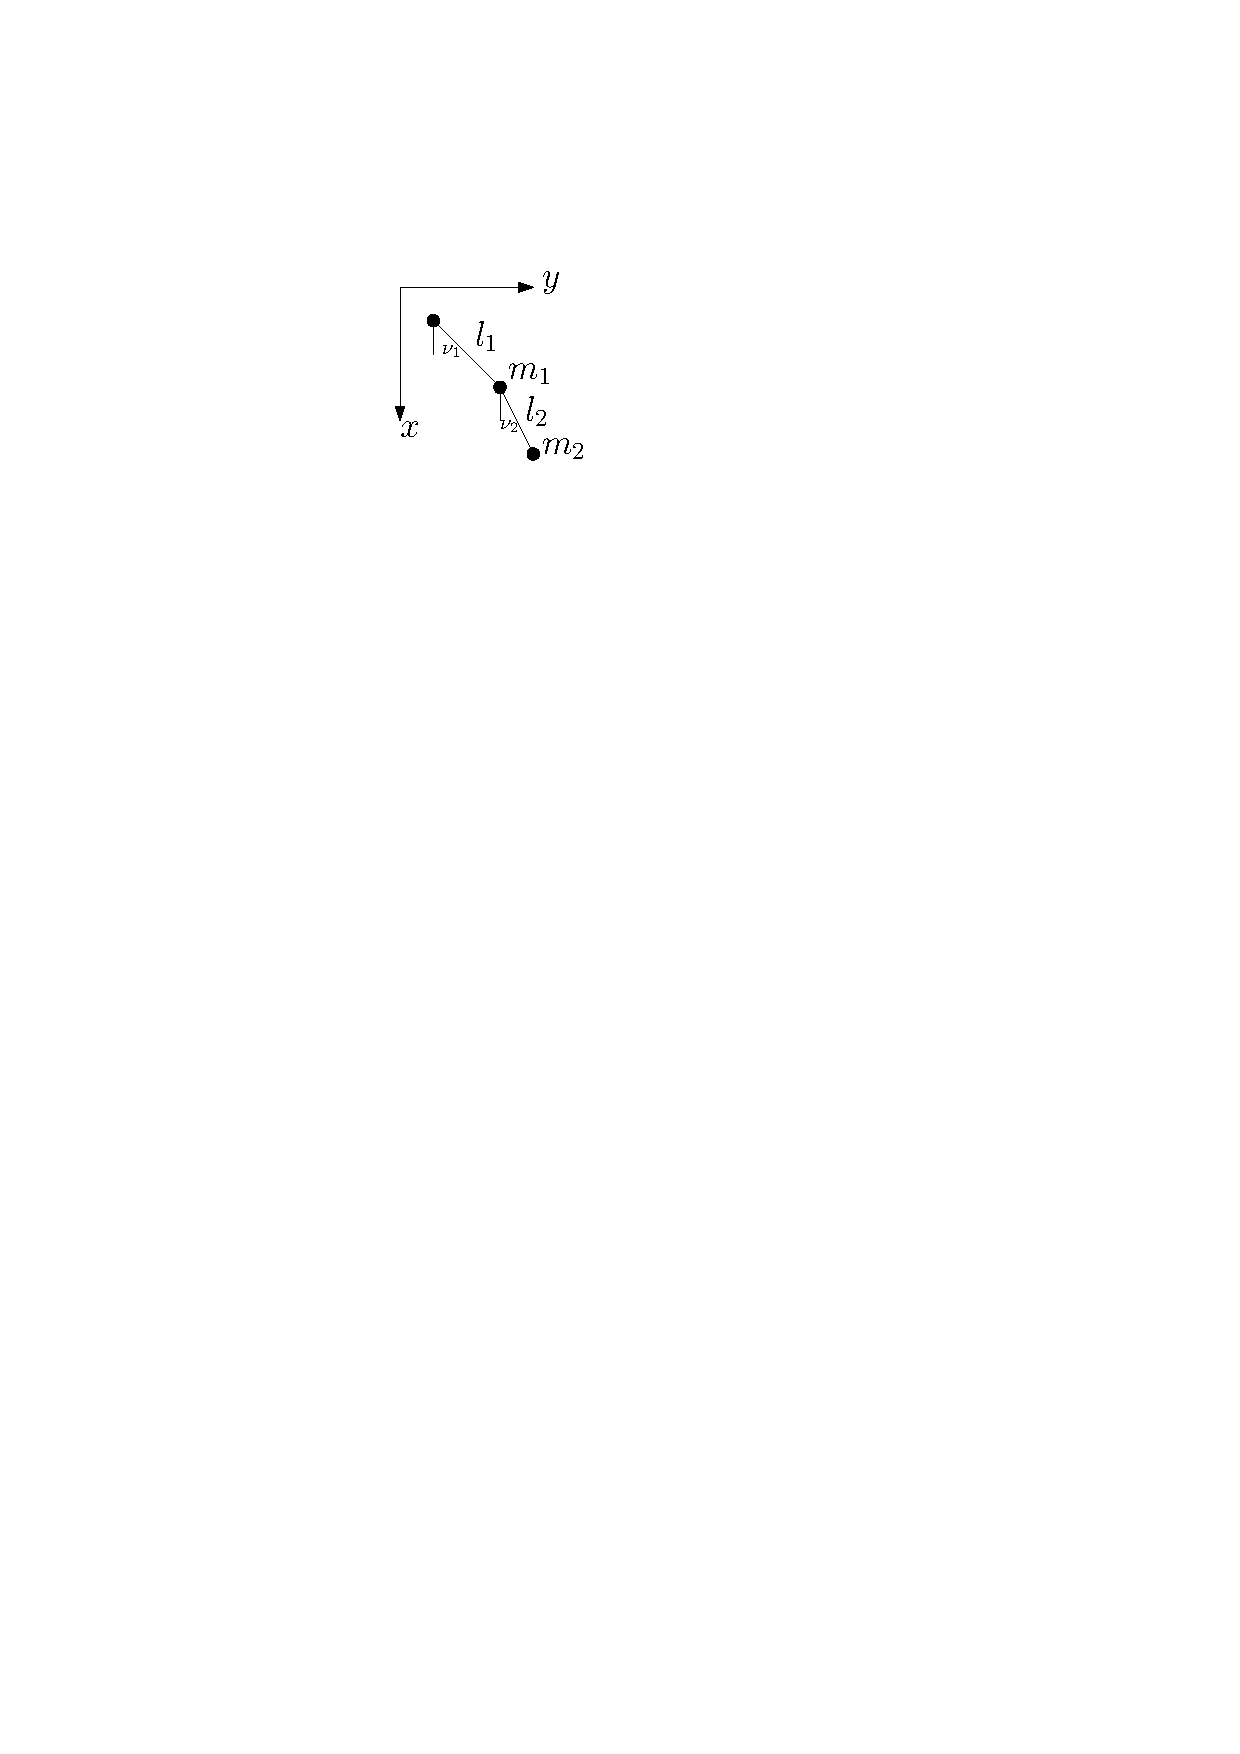
\includegraphics{figures/ch1/doppelpendel}
		\caption{Doppelpendel}
		\label{fig:ch1_doppelpendel}
	\end{figure}
\end{enumerate}


	
	\chapter{Übung 1}

\section*{Aufgabe 1}

\begin{description}
	\item[a)] 
	\[
		\frac{(a^2 - b^2)^{-2}}{(a + b)^{-3}} \cdot \frac{(a - b)^2}{a + b}
		= \frac{((a + b)(a - b))^{-2} (a - b)^2}{(a + b)^{-2}}
		= 1
	\] 
	
	\item[b)]
	\[
		\ln(e^{3x} e^{5x}) = \ln(e^{3x + 5x}) 
		= 8x
	\]
	
	\item[c)]
	\[
		\cos(\phi) + \sin(\phi) \tan(\phi) 
		= \frac{\cos^2(\phi)}{\cos(\phi)} \frac{\sin^2(\phi)}{\cos(\phi)}
		= \frac{1}{\cos(\phi)} 
	\]
\end{description}

\section*{Aufgabe 2}

\begin{description}
	\item[a)] 
	\[
		\sdiv{a \cos(x) + \sin(bx + c)}{x} = - a \sin(x) + \cos(bx + c) b
	\] 
	
	\item[b)]
	\[
		\sdiv{(3 + 2x - x^2)e^x}{x} = e^x (3 + 2x - x^2) + (2 - 2x)e^x = e^x (5 - x^2)
	\]
	
	\item[c)]
	\[
		\sdiv{(3 + 4x - x^2)^{1/2}}{x} = (3 + 4x - x^2)^{-1/2} (2 - x)
	\]
	
	\item[d)]
	\[
		\sdiv{x^x}{x} = x^x (\ln(x) + 1)
	\]
\end{description}

\section*{Aufgabe 3}
Die Ableitungen lauten
\begin{align*}
	g'(x) &= 3x^2 - 4x \\	
	g''(x) &= 6x - 4
\end{align*}
und es gilt $g'(x_0) = 0$ genau dann, wenn $x_0 = 0$ oder $x_0 = \frac{4}{3}$. Da $g''(0) = -4 < 0$ liegt dort ein Hochpunkt und da $g''(\frac{4}{3}) = 4 > 0$ liegt dort ein Tiefpunkt.

\section*{Aufgabe 4}
\begin{description}
	\item[a)] 
	\[
		F(x) = \int \frac{x^4 + 2x^2 - 5x + 1}{x} \mathrm{d}x
		= \int x^3 + 2x - 5 + \frac{1}{x} \mathrm{d}x
		= \frac{1}{4} x^4 + x^2 - 5x + \ln(x) + c	
	\]
	\item[b)]
	\begin{description}
		\item[i)] 
		\begin{align*}
			F 
			&= \int^2_1 \mathrm{d} x \ln(x) \int^\infty_{\ln(x)} \mathrm{d} y e^{-y}
			= \int^2_1 \ln(x) \left[ - e^{-y} \right]^\infty_{\ln(x)} \mathrm{d} x \\
			&= \int^2_1 \ln(x) e^{-\ln(x)} \mathrm{d} x
			= \frac{1}{2} \int^2_1 2 \ln(x) \frac{1}{x} \mathrm{d} x
			= \frac{1}{2} \left[ \ln^2(x) \right]^2_1
			= \frac{1}{2} \ln^2(x)
		\end{align*}
		
		\item[ii)] Kopf durch die Wand Methode:
		\[
			F(a) = \int^\infty_{-\infty} x e^{-ax^2} \mathrm{d} x 
			= \left[ -\frac{1}{2a} e^{-ax^2} \right]^\infty_{-\infty}
			= 0
		\]
		
		Kopf Methode: Die Funktion ist Punktsymmetrisch zum Ursprung, also Integral $=0$.
		
		\item[iii)] 
		\begin{align*}
			F(a) &= \int^\infty_{\infty} x^2 e^{-ax^2} \mathrm{d} x 
			= - \int^\infty_{-\infty} \left( \sdiv{}{a} e^{-ax^2} \right) \mathrm{d} x
			= -\sdiv{}{a} \int^\infty_{-\infty} e^{-ax^2} \mathrm{d} x
			= -\sdiv{}{a} \sqrt{\frac{\pi}{a}} \\
			&= \frac{\sqrt{\pi}}{2} a^{-3/2}
		\end{align*}
	\end{description}
\end{description}

\section*{Aufgabe 5}
\begin{description}
	\item[a)]
	\[
		AB - BA
		= \begin{pmatrix}
			1 & 7 \\ 6 & -6
		\end{pmatrix} + 
		\begin{pmatrix}
			6 & -2 \\ 1 & -5
		\end{pmatrix}
		= \begin{pmatrix}
			7 & 5 \\ 7 & -11
		\end{pmatrix}
	\] 
	
	\item[b)]
	\[
		\tr[AB - BA] = -4
	\]
	
	\item[c)]
	\[
		A^{-1} = \frac{1}{\det A} \begin{pmatrix}
			2 & -3 \\
			2 & 1
		\end{pmatrix}
		= \frac{1}{8} \begin{pmatrix}
			2 & -3 \\ 2 & 1
		\end{pmatrix}
	\]
\end{description}
	\chapter{Übung 2}

\section*{Aufgabe 1}

\begin{description}
	\item[a)] $f'(x) = x^3 + 2x - 5 + \frac{1}{x}$
	\item[b)] $f(x) = \cos(x) + \sin(x) \tan(x) = \frac{\cos^2(x)}{\cos(x)} + \frac{\sin^2(x)}{\cos(x)} = \frac{1}{\cos(x)}$, also $f'(x) =\sin(x) \frac{1}{\cos^2(x)} = \frac{\sin(x)}{\cos^2(x)} = \frac{\tan(x)}{\cos(x)}$
	\item[c)] $f(x) = \frac{1}{2 \sqrt{2}} \arctan\left( \frac{2 \sqrt{2}}{1 - x^2} \right)$
	
	Bronstein 6.1.22: $g(x) = \arctan(x)$ $\Rightarrow$ $g'(x) = \frac{1}{1 + x^2}$
	
	Damit: $f'(x) 
	= \frac{1}{2 \sqrt{x}} \frac{1}{1 + \frac{2x^2}{(1 - x^2)^2}} \sqrt{2} \frac{1 - x^2 + 2x^2}{(1 - x^2)^2}
	= \frac{1}{2} \frac{1 + x^2}{(1 - x)^2 + 2x^2}
	= \frac{1}{2} \frac{1 + x^2}{x^4 + 1}$
	
	\item[d)] $f(x) = \frac{1}{4 \sqrt{2}} \log \left( \frac{x^2 + \sqrt{2} x + 1}{x^2 - \sqrt{2}x + 1} \right)$
	
	$f'(x) 
	= \frac{1}{4 \sqrt{2}} \left( \frac{x^2 + \sqrt{2}x + 1}{x^2 - \sqrt{2}x + 1} \right)^{-1} \frac{(2x + \sqrt{2})(x^2 - \sqrt{2}x + 1)-(2x + \sqrt{2})(x^2 + \sqrt{2}x + 1)}{(x^2 + \sqrt{2}x + 1)^2}
	= \dots 
	= \frac{1}{2} \frac{1 - x^2}{x^4 + 1}$
\end{description}

\section*{Aufgabe 2}

\begin{description}
	\item[a)] $f(x) = \cos(x)$, $f'(x) = -\sin(x)$, $f''(x) = -\cos(x)$, also $f(0) = 1$, $f'(0) = 0$, $f''(0) = -1$.
	
	Damit ergibt sich: $f(x) = 1 + 0 x + \left( -\frac{1}{2} \right)x^2 + \mathcal{O}(x^3) \approx 1 - \frac{x^2}{2}$
	
	\item[b)] $f(x) = \log(1 - x)$, $f'(x) = -\frac{1}{1 - x} = \frac{1}{x - 1}$, $f''(x) = -\frac{1}{(x - 1)^2}$, also $f(0) = 0$, $f'(0) = 1$, $f''(0) = -1$.
	
	Damit ergibt sich: $f(x) = -x - \frac{x^2}{2} + \mathcal{O}(x^3)$.
\end{description}

\section*{Aufgabe 3}

\begin{description}
	\item[a)] $f(x) = e^{\lambda x} \sin(3x)$, man rechne:
	\begin{align*}
		\int e^{\lambda x} \sin(3x) \mathrm{d} x	
		&= \frac{1}{\lambda} e^{\lambda x} \sin(3x) - \frac{3}{\lambda} \int e^{\lambda x} \cos(3x) \mathrm{d} x \\
		&= \frac{1}{\lambda} e^{\lambda x} \sin(3x) - \frac{3}{\lambda} \left[ \frac{1}{\lambda} e^{\lambda x} \cos(3x) + \frac{3}{\lambda} \int e^{\lambda x} \sin(3x) \mathrm{d} x \right]
	\end{align*}
	
	Damit ergibt sich:
	\[
		\left( 1 + \frac{9}{\lambda^2} \right) \int e^{\lambda x} \sin(3x) \mathrm{d} x = \frac{1}{\lambda^2} e^{\lambda x} \left( \lambda \sin(3x) - 3 \cos(3x) \right)	
	\]
	
	Noch durch den Vorfaktor teilen:
	\[
		\int e^{\lambda x} \sin(3x) \mathrm{d} x 
		= \frac{1}{\lambda^2 + 9} e^{\lambda x} \left( \lambda \sin(3x) - 3 \cos(3x) \right) + C
	\]

	\item[b)] Stichwort: Partialbruchzerlegung
	\[ 
		\frac{1}{(1 - x)(1 + x)} 
		= \frac{A}{1 - x} + \frac{B}{1 + x} 
		= \frac{A + Ax + B - Bx}{(1 - x)(1 + x)} 
		= \frac{x(A - B) + (A + B)}{(x - 1)(x + 1)}
	\]
	Vergleich: $A = \frac{1}{2}$, $B = \frac{1}{2}$
	
	Nun einfach:
	\begin{align*}
		\int \frac{1}{(x - 1)(x + 1)} \mathrm{d} x 
		&= \int \frac{1}{2} \frac{1}{x - 1} + \frac{1}{2} \frac{1}{1 + x} \mathrm{d} x 
		= - \frac{1}{2} \log(1 - x) + \frac{1}{2} \log(1 + x) + C \\
		&= \frac{1}{2} \log \left( \frac{1 + x}{1 - x} \right) + C
	\end{align*}

	\item[b, i)] Verwende Substitution $x = \sin(z)$, $\frac{\mathrm{d} x}{\mathrm{d} z} = \cos(z)$, $z = \arcsin(x)$
	
	\begin{align*}
		\int_0^1 \frac{\mathrm{d} x}{\sqrt{1 - x^2}}	 
		&= \int^{\pi/2}_{0} \frac{1}{\sqrt{1 - \sin^2(z)}} \frac{\mathrm{d} x}{\mathrm{d} z} \mathrm{d} z
		= \int^{\pi / 2}_0 \frac{1}{\cos(z)} \cos(z) \mathrm{d} z
		= \int^{\pi / 2}_0 1 \mathrm{d} z \\
		&= \left[ z \right]^{\pi / 2}_0 = \frac{\pi}{2}
	\end{align*}

	\item[b, ii)]  $F(a, n) = \int^\infty_{-\infty} x^{2n} e^{-ax^2} \mathrm{d} x$ mit $a > 0$
	\begin{align*}
			F(a, n) 
			&= \left( \frac{\mathrm{d}}{\mathrm{d} a} \right)^n (-1)^n \int^{\infty}_{-\infty} e^{-ax^2} \mathrm{d} x
			= \left( \frac{\mathrm{d}}{\mathrm{d} a} \right)^n (-1)^n \sqrt{\frac{\pi}{a}} \\
			&=  \sqrt{\pi} \frac{\mathrm{d}^n}{\mathrm{d} a^n} \left( a^{-1/2} \right) (-1)^n
			= \sqrt{\pi} (-1)^n \frac{\mathrm{d}^{n -1}}{\mathrm{d} a^{n - 1}} \left( -\frac{1}{2} a^{-3/2} \right) \\
			&= \sqrt{\pi} (-1)^n \frac{\mathrm{d}^{n - 2}}{\mathrm{d} a^{n - 2}} \left( \frac{1}{2} \frac{3}{2} a^{-5/2} \right) 
			= \dots 
			= \sqrt{\pi} (-1)^n (-1)^n \left( \frac{1}{2} \frac{3}{2} \cdot \hdots \cdot \frac{2n - 1}{2} a^{-(2n + 1)/2} \right) \\
			&= \dots
	\end{align*}
\end{description}

\section*{Aufgabe 4}

\begin{description}
	\item[a)] 
	\begin{tabular}{|c||c|c|c|c|c|c|c|c|}
		\hline 
		$z = x + iy$ & $1 + 1i$ & $3 - 4i$ & $-3 + 2i$ & -2 & $5 - 12 i$ & $-1 - i$ & 1 + 1.7i \\
		\hline
		$r = \mabs{z}$ & $\sqrt{2}$ & $5$ & $\sqrt{13}$ & $2$ & $13$ & $\sqrt{2}$ & 2 \\
		\hline 
		$\phi = \arg(z)$ & $\frac{\pi}{4}$ & $1.705 \pi$ & $0.813 \pi$ & $\pi$ & $1.626 \pi$ & $\frac{5}{4} \pi$ & $-\pi/3$ \\
		\hline 
	\end{tabular}
 
	\item[b, i)] $z = \frac{1 + i}{2 + 3i} = \frac{(1 + i)(2 - 3i)}{(2 + 3i)(2 - 3i)} = \dots = \frac{5 - i}{13} \approx \frac{1}{13} \sqrt{26} e^{1.937 \pi i}$
	
	\item[b, ii)] $z = \frac{1}{\sqrt{1 + i}} = (1 + i)^{-1/2} = \left( \sqrt{2}\exp^{i \frac{\pi}{4}} \right)^{-1/2}$
	
		$z'_1 = 2^{-1/4} e^{-i \frac{\pi}{8} + 2 \pi i}$
		
		$z'_2 = 2^{-1/4} e^{-i \frac{9}{8} \pi + 2 \pi i}$
\end{description}
\end{document}

%%% Local Variables:
%%% mode: latex
%%% TeX-master: t
%%% End:
